% Chapter Template

\chapter{PubSeq Tagging Pipeline} % Main chapter title

\label{Chapter4} % Change X to a consecutive number; for referencing this chapter elsewhere, use \ref{ChapterX}

\lhead{Chapter 4. \emph{PubSeq tagging Pipeline}} % Change X to a consecutive number; this is for the header on each page - perhaps a shortened title

This chapters technically describes the whole routines of PubSeq Tagging Pipeline. Each single process will be presented and explained along with its program definitions and call arguments.

%----------------------------------------------------------------------------------------
%	SECTION 1
%----------------------------------------------------------------------------------------

\section{Introduction}

In this chapter, we would discuss various steps belonging to Tagging Pipeline. Following main steps belong to the Tagging Pipeline:

\begin{enumerate}
\item \textbf{Formatting} downloaded MEDLINE abstract into input files that are compliant with STRING  Tagger. \label{itm:TaggingStep1} (1)
\item \textbf{Named Entity tagging} done by STRING Tagger. \label{itm:TaggingStep2} (2)
\item \textbf{Post-processing} of the results and \textbf{preparation} for the entry into Solr index. \label{itm:TaggingStep3} (3)
\item \textbf{Updating} of results onto Solr Index. \label{itm:TaggingStep4} (4)
\end{enumerate}

The processes are then further divided into several single programs:

\begin{itemize}
\item \texttt{XMLAbstractsFormatter.java}
\item \texttt{tagcorpus.cxx}
\item \texttt{AnnotationBackmapper.java}
\item \texttt{Annotater.java}
\item \texttt{StatisticsUtils.java}
\item \texttt{IndexerNew.java}
\item \texttt{SolrUpdater.java}
\end{itemize}

The division of the whole pipeline into smaller tasks are reasoned through following arguments:
\begin{itemize}
\item The NER Tagger \ref{itm:TaggingStep2} was developed in C++ while we would implement the rest of pipeline (\ref{itm:TaggingStep1}, \ref{itm:TaggingStep3} and \ref{itm:TaggingStep4}) in Java. This means that pre- and post-tagging procedures would have to be implemented separately. Also since the NER Tagger wasn't written by us and therefore support would be very lacking, we would rather leave the NER Tagger as it is.
\item Related to previous argument: Solr is implemented in Java and its most comprehensive API (written by the developers of the Solr themselves) is written in Java \citep{grainger2014solr}. Therefore using Java in \ref{itm:TaggingStep4} would be almost necessary for various convenience reasons.
\item The pipeline generally is very memory intensive. During the process, several maps that each would gulp easily teens of gigabyte of memory are utilized. Therefore each step that utilizes such huge maps are all separated into one single routine.
\item Dividing the pipeline into smaller components would make it easy to debug, since each routine easily takes several minutes if not hours to run. However this also makes expanding features within the Tagging Pipeline more difficult.
\end{itemize}

Besides processes mentioned above, there is one process that doesn't exactly belong to Tagging Pipeline but is closely coupled and synchronized with it: downloading and storing of MEDLINE abstracts. Both download and maintenance of MEDLINE corpus and the Tagging pipeline would be covered in following sub-chapters.

As mentioned several times before, the Tagging Pipeline would be run every day in the morning in two steps: updating the MEDLINE corpus and the Tagging Pipeline itself. As the Tagging Pipeline concludes, all updates for the day that were fetched from MEDLINE leasing scheme server \citep{MEDLINE} would be indexed within Solr.

\begin{figure}[htbp]
    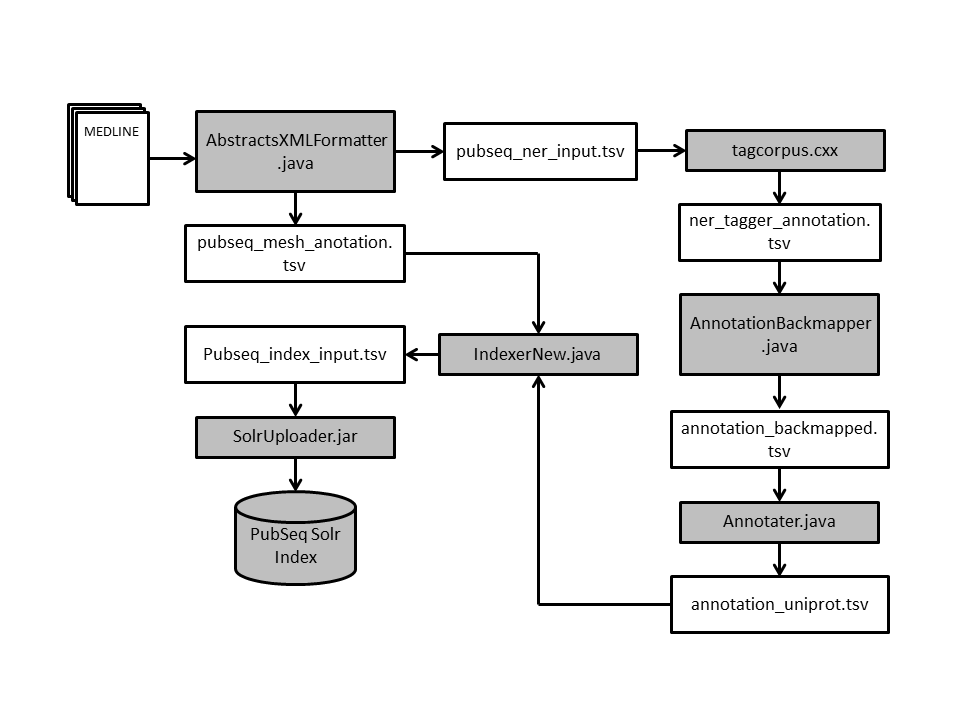
\includegraphics[width=6in]{Figures/tagging_pipeline_complete.png}
    \rule{35em}{0.5pt}
  \caption[(Resized) Overview of PubSeq Tagging Pipeline with all essential programs showed as nodes and important input/output files shown]{Overview of PubSeq Tagging Pipeline. Here we see how the raw data, MEDLINE XML file, is going through layers of program and ends up as input data for Solr Index. Here we also noticed that the workflow is structured as directed acyclic graph, where some data from non-immediate previous step would be used in later steps. The larger, original size of the workflow could be found in Appendix \ref{fig:PubSeqTaggingFull}}
  \label{fig:PubSeqTaggingComplete}
\end{figure}

%----------------------------------------------------------------------------------------
%	SECTION 2
%----------------------------------------------------------------------------------------

\section{MEDLINE Abstracts}

\label{sec:MEDLINEAbstracts}

We used NLM's leasing scheme \citep{MEDLINE} to retrieve the MEDLINE corpus. Each day, an updated from MEDLINE server is downloaded via FTP protocol onto our server. The update will happen daily at around 8 A.M. server time (CET/CEST). Each update is formatted as an XML file, each with an incrementing numerical identifier: the files are named \texttt{meldine15nXXXX.xml} with \texttt{XXXX} the integer identifier -- that is, the update file \texttt{meldine15n1057.xml} comes right after \texttt{meldine15n1056.xml} and before \texttt{meldine15n1058.xml}. The definition of MEDLINE XML file currently follows National Library of Medicine's (NLM) MEDLINE/PubMed Document Type Definition (DTD) \citep{MEDLINEDTD}, which at the time of thesis writing, is currently at the version dated 01/01/2015 \footnote{accessed 8/20/2015}.


Following is a slightly redacted example of a MEDLINE reference, which is taken for the paper by Karapakis-Liaskos and Ferrero, Nat. Rev. Immunol., 2015\footnote{doi:10.1038/nri3837}:

\label{lst:MEDLINEDTDExample}
\begin{lstlisting}[breaklines]
<MedlineCitation Owner="NLM" Status="In-Data-Review">
<PMID Version="1">25976515</PMID>
<DateCreated>
<Year>2015</Year>
<Month>05</Month>
<Day>26</Day>
</DateCreated>
<Article PubModel="Print-Electronic">
<Journal>
<ISSN IssnType="Electronic">1474-1741</ISSN>
<JournalIssue CitedMedium="Internet">
<Volume>15</Volume>
<Issue>6</Issue>
<PubDate>
<Year>2015</Year>
<Month>Jun</Month>
</PubDate>
</JournalIssue>
<Title>Nature reviews. Immunology</Title>
<ISOAbbreviation>Nat. Rev. Immunol.</ISOAbbreviation>
</Journal>
<ArticleTitle>Immune modulation ... membrane vesicles.</ArticleTitle>
<Pagination>
<MedlinePgn>375-87</MedlinePgn>
</Pagination>
<ELocationID EIdType="doi" ValidYN="Y">10.1038/nri3837</ELocationID>
<Abstract>
<AbstractText>Gram-negative ... nanotechnologies.</AbstractText>
</Abstract>
<AuthorList CompleteYN="Y">
<Author ValidYN="Y">
<LastName>Kaparakis-Liaskos</LastName>
<ForeName>Maria</ForeName>
<Initials>M</Initials>
<AffiliationInfo>
<Affiliation>MIMR-PHI Institute of ..., Australia.</Affiliation>
</AffiliationInfo>
</Author>
<Author ValidYN="Y">
<LastName>Ferrero</LastName>
<ForeName>Richard L</ForeName>
<Initials>RL</Initials>
<AffiliationInfo>
<Affiliation>MIMR-PHI Institute of ..., Australia.</Affiliation>
</AffiliationInfo>
</Author>
</AuthorList>
<Language>eng</Language>
<PublicationTypeList>
<PublicationType UI="D016428">Journal Article</PublicationType>
</PublicationTypeList>
<ArticleDate DateType="Electronic">
<Year>2015</Year>
<Month>05</Month>
<Day>15</Day>
</ArticleDate>
</Article>
<MedlineJournalInfo>
<Country>England</Country>
<MedlineTA>Nat Rev Immunol</MedlineTA>
<NlmUniqueID>101124169</NlmUniqueID>
<ISSNLinking>1474-1733</ISSNLinking>
</MedlineJournalInfo>
<CitationSubset>IM</CitationSubset>
</MedlineCitation>
\end{lstlisting}

%----------------------------------------------------------------------------------------
%	SUBSECTION 2.1
%----------------------------------------------------------------------------------------

\subsection{Specifications}

\begin{table}[htbp]
\caption{Specifications table for PubSeq MEDLINE Abstracts}
\centering
\begin{tabular}{ | l | l | }
  \hline
  Parameter & Value \\
  \hline
  URL, repo & none \\
  Path, clone & none \\
  Path, running program & \texttt{/mnt/project/rost\_db/medline}\\
  \hline
\end{tabular}
\end{table}

%\begin{figure}[!h]
%	\theverbbox
%\caption{An example of a reference from XML MEDLINE corpus}
%\label{fig:singlecell_chemo}
%\end{figure}

%----------------------------------------------------------------------------------------
%	SECTION 3
%----------------------------------------------------------------------------------------

\section{XMLAbstractFormatter.java}

\label{sec:XMLAbstractFormatter}

This class represents a formatter that parses the MEDLINE abstract files and transforms it into STRING Tagger-compliant format. It follows NLM DTD for MEDLINE \citep{MEDLINEDTD} as parsing reference. In the directory where the updates were downloaded, it lists down all possible XML files and parses files that had not been processed before. For each XML file, it creates a tree representation of the file through full. Owning to its tree-like structure \citep{bray2011extensible} \citep{MEDLINEDTD}, this implies that each \texttt{MedlineCitation} tag is itself is a tree (see Section \ref{lst:MEDLINEDTDExample}) . For each \texttt{MedlineCitation} it extracts needed information such as PubMed ID, title, journal name, publication date, abstract, authors and associated MeSH IDs \citep{lowe1994understanding} and writes it out.

\subsection{Parameters}

\begin{lstlisting}[breaklines]
path_to_medline ner_output_path mesh_output_path counter_file counter_max
\end{lstlisting}

\begin{itemize}
\item \texttt{path\_to\_medline}: the location of MEDLINE xml abstracts. The program will recursively traverse all sub directories of this path and parse files matching following name pattern: \texttt{meldine15nXXXX.xml}.

\item \texttt{ner\_output\_path}: path the first output file (with name) should be written onto. The first output file would then be used for Tagging by PubSeq NER Tagger.

\item \texttt{mesh\_output\_path }: to path the second output file (with name) should be written onto. The second output file contains associative table between PMID and list of MeSH IDs associated with the publication. Since STRING Tagger input is fixed we write this information in separate file.

\item \texttt{counter\_file}: file containing the location of last parsing. The program parses \texttt{XXXX} of the name format and figures whether current integer is larger than the one written in \texttt{counter\_file} before parsing the content of the update file. Upon the completion of the run, the program will replace the value within \texttt{counter\_file} with the largest \texttt{XXX} it encountered. This would be then the starting point of the next run.

\item \texttt{counter\_max}: file containing the maximum \texttt{XXXX} this program should read. If \texttt{counter\_file} contains 1000 and \texttt{counter\_max} 1500 it will only parse \texttt{meldine15n1001.xml} all the way through \texttt{meldine15n1500.xml} in this run. Note that \texttt{counter\_max} is not updated after run. If \texttt{counter\_max} doesn't exist in system then the it assumes \texttt{Integer.MAX\_VALUE} \footnote{\href{http://docs.oracle.com/javase/7/docs/api/java/lang/Integer.html}{\texttt{http://docs.oracle.com/javase/7/docs/api/java/lang/Integer.html}}, accessed 08/20/2015} as upper bound of the parsing.
\end{itemize}

\subsection{Specifications}

\begin{table}[htbp]
\caption{Specifications table for XMLAbstractsFormatter.java}
\centering
\begin{tabularx}{\textwidth}{ | l | X | }
  \hline
  Parameter & Value \\
  \hline
  URL, repo & See Appendix \ref{AppendixA} \\
  Path, clone & \texttt{/mnt/project/pubseq/dev/pubseq-tagging /PubSeq/src/org/pubseq/utils/ XMLAbstractsFormatter.java} \\
  Path, running program & \texttt{/mnt/project/pubseq/dev/pubseq-tagging /PubSeq/src/org/pubseq/utils/ XMLAbstractsFormatter.java} \\
  \hline
\end{tabularx}
\end{table}

%----------------------------------------------------------------------------------------
%	SECTION 4
%----------------------------------------------------------------------------------------

\section{tagcorpus.cxx}

This program is the core component of our Tagging Pipeline. It takes a tab-separated file as input and tags various entities within each abstract. Originally developed by Jensen et al at University of Copenhagen, the backbone of the program is based in NER tagging environment that was used in (Pacifilis, et al, 2013 \citep{pafilis2013species}), which in turn utilizes dictionaries curated within the framework of STRING database (Szklarczyk, et al, 2011 \citep{szklarczyk2011string}).

In very broad explanation, the program uses various kind of mapping for various entities. While parsing a text, the program checks for word combinations that looks similar to the entries that were mapped (i.e. the word has small Levensthein distance \citep{levenshtein1966binary} to some word within the map). For an NER program, the program is astonishingly fast. A full set of MEDLINE corpus with ca. 26 million articles could be parsed in under 12 hours (the mileage may vary according to server specification and number of threads involved).

Our entry point into the program is \texttt{tagcorpus.cxx}. There are several modi of running the program. However, in the modus that we use to tag MEDLINE abstracts, we call the tagger in following manner:


\begin{lstlisting}[breaklines]
input_file | path_to_named_entity_tagger/tagcorpus path_to_pubseq_programdata/entities.tsv path_to_named_entity_tagger_data/names.tsv path_to_named_entity_tagger_data/global.tsv path_to_named_entity_tagger_data/local.tsv path_to_named_entity_tagger_data/groups.tsv > output_file_path
\end{lstlisting}

\begin{itemize}
\item \texttt{input\_file} is the formatted input from \texttt{XMLAbstractsFormatter.java}.
\item \texttt{path\_to\_named\_entity\_tagger/tagcorpus}: the location of compiled binary \texttt{tagcorpus.cxx}, our gateway to the program. See Appendix \ref{AppendixA} for the detail of program structure.
\item \texttt{path\_to\_pubseq\_programdata/entities.tsv}: the location of table \texttt{entities.tsv}.
\item \texttt{path\_to\_pubseq\_programdata/names.tsv}: the location of table \texttt{names.tsv}.
\item \texttt{path\_to\_pubseq\_programdata/global.tsv}: the location of table \texttt{global.tsv}.
\item \texttt{path\_to\_pubseq\_programdata/local.tsv}: the location of table \texttt{local.tsv}.
\item \texttt{path\_to\_pubseq\_programdata/groups.tsv}: the location of table \texttt{groups.tsv}.
\end{itemize}

While there are several input files besides the prepared MEDLINE abstracts file itself, there are only four tables that we are mainly concerned with: the MEDLINE input table itself, \texttt{entities.tsv}, \texttt{names.tsv} and the output table.

\subsection{MEDLINE Input Table}

The NER Tagger takes a tab-separated table with following format as input:

\begin{itemize}
\item first column: PMID of the article with format of \texttt{PMID:article\_pmid}.
\item second column: list of authors. Each author is separated with semicolon.
\item third column: journal name.
\item fourth column: publication date.
\item fifth column: title.
\item sixth column: abstract.
\end{itemize}

Following is an example of valid input line, taken for the paper by Gu, et al, The Journal of Cell Biology, 1999 \footnote{doi: 10.1083/jcb.147.5.1085}:


\begin{lstlisting}[breaklines]
10579727	M Gu;X Xi;G D Englund;M C Berndt;X Du	The Journal of cell biology	1999-11-29T00:00:01Z	Analysis of the roles of 14-3-3 in the platelet glycoprotein Ib-IX-mediated activation of integrin alpha(IIb)beta(3) using a reconstituted mammalian cell expression model.	We have reconstituted the platelet glycoprotein (GP) Ib-IX-mediated activation of the integrin alpha(IIb)beta(3) in a recombinant DNA expression model, and show that 14-3-3 is important in GPIb-IX signaling. CHO cells expressing alpha(IIb)beta(3) adhere poorly to vWF. Cells expressing GPIb-IX adhere to vWF in the presence of botrocetin but spread poorly. Cells coexpressing integrin alpha(IIb)beta(3) and GPIb-IX adhere and spread on vWF, which is inhibited by RGDS peptides and antibodies against alpha(IIb)beta(3). vWF binding to GPIb-IX also activates soluble fibrinogen binding to alpha(IIb)beta(3) indicating that GPIb-IX mediates a cellular signal leading to alpha(IIb)beta(3) activation. Deletion of the 14-3-3-binding site in GPIbalpha inhibited GPIb-IX-mediated fibrinogen binding to alpha(IIb)beta(3) and cell spreading on vWF. Thus, 14-3-3 binding to GPIb-IX is important in GPIb-IX signaling. Expression of a dominant negative 14-3-3 mutant inhibited cell spreading on vWF, suggesting an important role for 14-3-3. Deleting both the 14-3-3 and filamin-binding sites of GPIbalpha induced an endogenous integrin-dependent cell spreading on vWF without requiring alpha(IIb)beta(3), but inhibited vWF-induced fibrinogen binding to alpha(IIb)beta(3). Thus, while different activation mechanisms may be responsible for vWF interaction with different integrins, GPIb-IX-mediated activation of alpha(IIb)beta(3) requires 14-3-3 interaction with GPIbalpha.
\end{lstlisting}

\subsection{entities.tsv}

\texttt{entities.tsv} is a three-column tsv table listing down all unique entity that is taggable by the program. Entity is the smallest unit from speech that is differential from each other. While being the smallest, an entity comes in many forms, with each lexically identifiable with each other. For example, \textit{United States of America}, \textit{America} and \textit{USA} belong to the same entity and are differentiable from \textit{France}, \textit{Republic of France} and \textit{French Republic}, all of which are identifiable with each other and belong to same entity. In STRING Tagger environment, we used STRING ID \citep{szklarczyk2011string} as our identifier \textit{within the Tagger} -- not to be confused with UniProt ID as unique protein identifier in PubSeq system.


Each of three column is defined as follows:


\begin{itemize}
\item first column: the STRING ID of an entity. STRING ID is unique identifier of each entity within STRING Tagger environment. An entity could be understood as one single unique named-entity that is recognizable in text (see explanation bellow).
\item second column: the designation of entity within NCBI Taxonomy Browser \footnote{\href{http://www.ncbi.nlm.nih.gov/taxonomy}{\texttt{http://www.ncbi.nlm.nih.gov/taxonomy}}, accessed 23/08/2015} \citep{federhen2012ncbi}. Since NER Tagger tags various kind of named-entity from protein to disease names, each kind of tag has to be assigned to an identifier describing what kind of named-entity does one entity belong to. A gene/protein belonging to human, for example, will be assigned value of 9606 \footnote{\href{http://www.ncbi.nlm.nih.gov/taxonomy/?term=9606}{\texttt{http://www.ncbi.nlm.nih.gov/taxonomy/?term=9606}}, accessed 23/08/2015}.
\item third column: the representation of this entity in alphanumeric form. The name which appears in this entry would be referred as \textbf{standard name} in later parts.
\end{itemize}

As explained before, a single entity could map to multiple written values. This mapping is described in another table, \texttt{names.tsv}.

\subsection{names.tsv}

\texttt{names.tsv} is mapping table between STRING ID (see the definition for \texttt{entites.tsv} above) and all its written forms. There are two columns in this table:

\begin{itemize}
\item first column: the STRING ID.
\item second column: the name of the entity.
\end{itemize}

As expected, the relation of this table is \textbf{1 x N}, that is, each of the element on the right is associated with only one element of the right and each of the elements on the left is associate with N elements on the right. Also, for each String ID from table entities.tsv, the entry from the third column of the table is also contained in \texttt{names.tsv}.

\subsection{STRING Tagger Annotation}

After finishing the tagging process, the NER Tagger would produce a file that lists down all annotations that it found. The output file is tab-separated, with each row representing a single annotation. There are 8 columns in the table:

\begin{itemize}
\item first column defines the PMID on which this annotation is found.
\item second column defines the start of internal ordering of annotation within STRING Tagger.
\item third column defines the end of internal ordering of annotation within STRING Tagger.
\item fourth column defines the start offset of the annotation within the input text.
\item fifth column defines the end offset of the annotation within the input text, inclusive.
\item sixth column defines tagged string as it appears in the input text.
\item seventh column defines designated associated taxonomy of entities the string is annotated with (see second column of \texttt{entities.tsv}).
\item eighth column defines the STRING ID of the entity the string is annotated with (see first column of \texttt{entities.tsv}.
\end{itemize}

As expected, the eight and ninth columns of the output file are coupled. Note also that a string within input text could be annotated with multiple entities. The reason for this is because since the string found in input text is likely to be ambiguous and has therefore to be tagged with multiple entities. To take as an example, \textit{America} could mean both \textit{United States of America} and the continent. Also given the enormous size of entities within \texttt{entities.tsv}, combinatorically the likelihood that two entities posses very similar written forms could not be trivialized.

%----------------------------------------------------------------------------------------
%	SECTION 5
%----------------------------------------------------------------------------------------

\section{AnnotationBackmapper.java}

\label{sec:AnnotationBackmapper}

This class modifies the results from STRING Tagger. The program AnnotationBackmapper.java does following task:

\begin{itemize}
\item Backmapping of the annotations (see bellow).
\item Computing statistics of the number of articles with annotation and the number of annotations. Note that the annotations taken statistics of include all possible kind of annotations that the NER tagging done (i.e. not only protein annotation)
\end{itemize}

The main task of this program is to map the sixth column of each of the NER Tagger annotations back to the name as it appears in entities.tsv. That is, given a result:

\begin{verbatim}
12345	1	1	11	13	some annotation	9606	23456789
\end{verbatim}

and the entry of \texttt{23456789} within \texttt{entities.tsv}:

\begin{verbatim}
23456789	9606	standard name
\end{verbatim}

this program replaces \texttt{some annotation} with \texttt{standard name}:

\begin{verbatim}
12345	1	1	11	13	standard name	9606	23456789
\end{verbatim}

This mapped back would be used in later part of the Tagging Process. Also knowing the standard name would help in development process and sanity check, since standard name is usually (in case of protein) unique within some databases (for example, most proteins have ENSEMBL ID as its standard name), albeit not uniformly -- the identifiers hailed from various systems including ENSEBML \citep{hubbard2002ensembl}, VectorBase \citep{lawson2009vectorbase} and some even have ordered locus (OLS) name as identifier \footnote{\href{http://www.uniprot.org/help/gene_name}{\texttt{http://www.uniprot.org/help/gene\_name}}, accessed 23/08/2015}.

\subsection{Parameters}

\begin{lstlisting}[breaklines]
ner_annotations entities_table result_path statistics_path
\end{lstlisting}

\begin{itemize}
\item \texttt{ner\_annotations}: the result of STRING Tagger.
\item \texttt{entities\_table}: the table as appeared in STRING Tagger.
\item \texttt{results\_path}: the path the backmapped annotations are to be written to.
\item \texttt{statistics\_path}: the file the statistics is to be written to.
\end{itemize}

\subsection{Specifications}

\begin{table}[htbp]
\caption{Specifications table for AnnotationBackmapper.java}
\centering
\begin{tabularx}{\textwidth}{ | l | X | }
  \hline
  Parameter & Value \\
  \hline
  URL, repo & See Appendix \ref{AppendixA} \\
  Path, clone & \texttt{/mnt/project/pubseq/pandu/pubseq-crawler/PubSeq /src/org/pubseq/annotation /AnnotationBackmapper.java} \\
  Path, running program & \texttt{/mnt/project/pubseq/pandu/pubseq-crawler/PubSeq /src/org/pubseq/annotation /AnnotationBackmapper.class}\\
  \hline
\end{tabularx}
\end{table}

%----------------------------------------------------------------------------------------
%	SECTION 6
%----------------------------------------------------------------------------------------

\section{Annotater.java}

This program "annotates" the tagging results of the NER tagger. Given a result row from NER Tagger, it checks whether the annotation is protein annotation -- if so, it then tries to find all UniProt IDs that this annotation maps to. As described before, every single annotation from NER tagger is associated with STRING ID and each STRING ID is described in \texttt{entities.tsv} with a standard name. This is also the case for protein annotation, it is associated with some identifier as standard name. The identifiers used are, however, not strucrtured and belong to single identifying system such as UniProt ID or ENSEMBL (see Section \ref{sec:AnnotationBackmapper}). This might seem problematic as the start since we decided to only use UniProt ID as standard and unique identifier for proteins. The NER Tagger however, provides such mapping implicitly. As explained in previous chapters, the table \texttt{names.tsv} maps each String ID to list of names it is associated with. Within the context of protein entity, each of the STRING ID maps to various names and other identifiers associated with this STRING ID, among others the UniProt IDs. We therefore had to merged these two tables with regard to the String ID and create a new table that maps standard name (that is, name that appears with STRING ID within table \texttt{entities.tsv} to other names that are associated with the same STRING ID. This step fortunately has been done in other step and belongs to the Maintenance Pipeline.

As thus, the program only has to parse the resulting merged table from the Maintenance Pipeline and maps the sixth column (already in standard name, see Section \ref{sec:AnnotationBackmapper}) to the list of all associated names. For each of associated names, an entry is written to output file in format similar to the output format of NER tagger with the sixth column replaced with associated names. That is, for each backmapped annotation from previous step:

\begin{verbatim}
12345	1	1	11	13	standard name	9606	23456789
\end{verbatim}

we checked whether standard name is a UniProt ID. If so, then we write this to output file. Otherwise we check whether there exists some mapping from standard name to list of names within the merged files. If there is one, write for each values the same entry with sixth column replaced:

\begin{verbatim}
12345	1	1	11	13	uniprot_id_1	9606	23456789
...
12345	1	1	11	13	uniprot_id_m	9606	23456789
\end{verbatim}


The multiple mapping of standard name to multiple UniProt IDs could be explained best by the fact that named-entity tagging is prone with lexical ambiguity \citep{ratinov2009design}. A protein named X might have associated with several entries in UniProt database, each with exact or almost exact assigned name. This is especially true in case of unreviewed proteins. There are for example several cases of UniProt entry named \textit{Brain-derived neurotrophic factor} (BNDF) \footnote{\href{http://www.uniprot.org/uniprot/?query=Brain-derived+neurotrophic+factor&sort=score}{\texttt{http://www.uniprot.org/uniprot/?query=Brain-derived+neurotrophic+factor\&sort=score}}, accessed 23/08/2015}. All aforementioned entries are both lexically and ideolexically the same -- they represent very similar things that have very similar name, which would be very hard to disambiguate \citep{ratinov2009design}. This is moreover exacerbated by the fact that many unreviewed proteins have names that are similar or exactly similar to the to the ones that are already reviewed. Looking at context around the annotation location might help to determine whether a named-entity belong to protein or not or whether a tagged protein name belongs to human or not (for example, by looking at whether the sentence/paragraph/paper delves into human disaese etc), however, exactly named protein belonging to same species is hard to differentiate by looking at text. Therefore the multiple mapping.

\subsection{Parameters}

\begin{lstlisting}[breaklines]
ner_backmapped_annotation merged_table uniprot_kbid output_file
\end{lstlisting}

\begin{itemize}
\item \texttt{ner\_backmapped\_annotation}: the result of previous step
\item \texttt{merged\_table}: the merged-filtered table created from \texttt{entities.tsv} and \texttt{names.tsv} (see program description above).
\item \texttt{uniprot\_kbid}: the mapper between UniProt Accession ID and its associated UniProtKB ID \footnote{ \href{ftp://ftp.uniprot.org/pub/databases/uniprot/current_release/knowledgebase/idmapping/}{\texttt{ftp://ftp.uniprot.org/pub/databases/uniprot/current\_release/knowledgebase/idmapping/}}, accessed 23/08/2015}. We use this as a reference for the full list of existing UniProt ID.
\end{itemize}

\subsection{Specifications}

\begin{table}[htbp]
\caption{Specifications table for Annotater.java}
\centering
\begin{tabularx}{\textwidth}{ | l | X | }
  \hline
  Parameter & Value \\
  \hline
  URL, repo & See Appendix \ref{AppendixA} \\
  Path, clone & \texttt{/mnt/project/pubseq/pandu/pubseq-crawler/PubSeq /src/org/pubseq/annotation/Annotater.java} \\
  Path, running program & \texttt{/mnt/project/pubseq/pandu/pubseq-crawler/PubSeq /src/org/pubseq/annotation/Annotater.class}\\
  \hline
\end{tabularx}
\end{table}

%----------------------------------------------------------------------------------------
%	SECTION 7
%----------------------------------------------------------------------------------------

\section{StatisticsUtils.java}


This step is mostly deprecated but is still connected with other program. It was initially intended as statistics mechanism that produces some descriptive statistics on the landscape of annotation for the whole MEDLINE abstract. Since the Tagging Pipeline is done regularly now, this method is not necessary for the whole pipeline.

\subsection{Specifications}

\begin{table}[htbp]
\caption{Specifications table for StatisticsUtils.java}
\centering
\begin{tabularx}{\textwidth}{ | l | X | }
  \hline
  Parameter & Value \\
  \hline
  URL, repo & See Appendix \ref{AppendixA} \\
  Path, clone & \texttt{/mnt/project/pubseq/pandu/pubseq-crawler/PubSeq /src/org/pubseq/utils/StatisticsUtils.java} \\
  Path, running program & \texttt{/mnt/project/pubseq/pandu/pubseq-crawler/PubSeq /src/org/pubseq/utils/StatisticsUtils.class}\\
  \hline
\end{tabularx}
\end{table}

%----------------------------------------------------------------------------------------
%	SECTION 8
%----------------------------------------------------------------------------------------

\section{IndexerNew.java}

\texttt{IndexerNew.java} is the last step before pushing the input data onto Solr index. The main purpose of this step is to put all information that were acquired during the Tagging Pipeline together. There are three kinds of information that we are particularly interested in form our pipeline:

\begin{itemize}
\item List of proteins that are mentioned in an article
\item List of taxonomy association of the proteins in the article
\item List of MeSH IDs of the article
\end{itemize}

The first information was obtained during NER Tagging process, while the latter two were obtained while parsing raw MEDLINE XML input. We will use the initially formatted MEDLINE file (see Section \ref{sec:XMLAbstractFormatter} bellow) as the template. The three kinds of information will each occupy one new column in the updated file. Hence, there would be then nine columns in the output file:

\begin{itemize}
\item first column: PMID of the article. Unlike the output format of \texttt{XMLAbstractFormatter.java}, the PMID will appear in plain ID form without the prefix \texttt{PMID:}).
\item second column: list of authors. Each author is separated with semicolon.
\item third column: journal name as appeared in XML input file.
\item fourth column: publication date.
\item fifth column: article title.
\item sixth column: article abstract. Multi-abstracts (i.e. abstracts with sub-organizations such as introduction, methods, results etc) would be represtented as one string.
\item seventh column: list of UniProt ID mentions, separated by space.
\item eight column: list of MeshID associated with the article, separated by space.
\item ninth column: unique list of UniProt ID species associations, separated by space.
\end{itemize}

To achieve, this, we initialized a map for each of the information, with PMIDs as key and the list of UniProt IDs/unique species/MeSH IDs as value. We do this by simply parsing the results from previous steps that contain the information we'd like to index:

\begin{itemize}
\item \textbf{List of UniProt ID Mentions} are available from post-processed NER tagger annotations. We use the output of Annotater.java. The program implements the index as Hash Map with PMID as key and list of UniProt as values. The file will be parsed sequentially and the UniProt ID annotation (sixth column) for the PMID (first column) would be pushed into the map. At the end, a temporary file will be written with added column created from this index. Upon embedding the merging will done and the result written. Afterwards, the map is deleted to free up memory.
\item \textbf{List of MeSH IDs} are available from \texttt{XMLAbstractFormatter.java}. Since the file is already in form of implicit map (two columns with first column containing PMID and second list of MeSH), the program just parses the file sequentially into the index. The later steps follow roughly the one for UniProt ID mentions.
\item \textbf{List of Species Associations} are available from post-processed NER tagger annotation. As reader can see in the output format of PubSeq NER Tagger, the seventh column contains the taxonomy association of the annotation. As such, this step follows closely the first procedure (List of UniProt ID mentions). The only different would be that the parser uses seventh instead of sixth column as value.
\end{itemize}

he reason behind doing this sequentially is, again, memory. In the worst case when the program has to index the whole MEDLINE abstract, memory usage for each of the step easily exceeds 20 GB. As such sequential steps were used instead of all-in-one approach.

\subsection{Parameters}

\begin{lstlisting}[breaklines]
template_path template_index_col_num output_dir_path first_file_path first_file_index_col_num first_file_value_col_num second_file_path second_file_index_col_num second_file_value_col_num third_file_path third_file_index_col_num third_file_value_col_num final_name
\end{lstlisting}

\begin{itemize}
\item \texttt{template\_path}: path to template file.
\item \texttt{template\_index\_col\_num}: column number of template file's reference column (PMID). This will be used for embedding template with additional columns.
\item \texttt{output\_dir\_path}: the directory where interim and final values are to be stored.
\end{itemize}

For each of the three files:

\begin{itemize}
\item \texttt{path}: output file path.
\item \texttt{index\_col\_num}: column number of the file's reference column (PMID).
\item \texttt{value\_col\_num}: column number of the file's value.
\end{itemize}

Also,

\begin{itemize}
\item \texttt{final\_name}: final name of the output file.
\end{itemize}

\subsection{Specifications}

\begin{table}[htbp]
\caption{Specifications table for IndexerNew.java}
\centering
\begin{tabularx}{\textwidth}{ | l | X | }
  \hline
  Parameter & Value \\
  \hline
  URL, repo & See Appendix \ref{AppendixA} \\
  Path, clone & \texttt{/mnt/project/pubseq/pandu/pubseq-crawler/PubSeq /src/org/pubseq/utils/IndexerNew.java} \\
  Path, running program & \texttt{/mnt/project/pubseq/pandu/pubseq-crawler/PubSeq /src/org/pubseq/utils/IndexerNew.class}\\
  \hline
\end{tabularx}
\end{table}

%----------------------------------------------------------------------------------------
%	SECTION 9
%----------------------------------------------------------------------------------------

\section{IndexerNew.java}

The class from which SolrUpdater.jar derives from, \textbf{SolrUpdater.java}, consists of module that will push new documents (Solr term for an entry) onto the index. Given the input table with updated columns from IndexerNew.java, this programs parses and pushes each row from the input. For each row from the input, the program checks whether such document already exists in the Solr index. If such document exists, it updates the attributes of existing document by adding new values coming from the parsed row. Otherwise, the program creates a document instance containing the values from parsed row as attributes. The document instance would then be pushed onto the index. The whole process utilizes the Solr native API for Java, SolrJ \citep{grainger2014solr} \footnote{\href{https://wiki.apache.org/solr/Solrj}{\texttt{https://wiki.apache.org/solr/Solrj}}, accessed 23/08/2015} \footnote{\href{https://cwiki.apache.org/confluence/display/solr/Using+SolrJ}{\texttt{https://cwiki.apache.org/confluence/display/solr/Using+SolrJ}}, accessed 23/08/2015}.

\subsection{Parameters}

\begin{lstlisting}[breaklines]
abstract_output_path index_url
\end{lstlisting}

\begin{itemize}
\item \texttt{abstract\_output\_path}: path of directory containing input table.
\item \texttt{index\_url}: URL on which the PubSeq core is accessible from see Chapter \ref{Chapter5} for the description of core within Solr environment. The URL of a core within an environment is basically a subpage of the index itself. That is, for an index located at \texttt{http://localhost:8983/solr/}, the address of core named \texttt{pubseq} would be \texttt{http://localhost:8983/solr/pubseq/}.
\end{itemize}

\subsection{Specifications}

\begin{table}[htbp]
\caption{Specifications table for SolrUploader.java}
\centering
\begin{tabularx}{\textwidth}{ | l | X | }
  \hline
  Parameter & Value \\
  \hline
  URL, repo & See Appendix \ref{AppendixA} \\
  Path, clone & \texttt{/mnt/project/pubseq/pandu/pubseq-crawler/PubSeq /src/org/pubseq/utils/SolrUploader.java} \\
  Path, running program & \texttt{/mnt/project/pubseq/pandu/pubseq-crawler/PubSeq /SolrUploader.jar}\\
  \hline
\end{tabularx}
\end{table}